\subsection{Result analysis}\label{Subsec:results}
The results of each test will in this section be compared to the baseline RMSE as seen in \autoref{fig:base_errors}, and with the RMSE score of the different methods.


\begin{figure}[H]
	\centering
	\begin{adjustbox}{width=0.5\textwidth}
		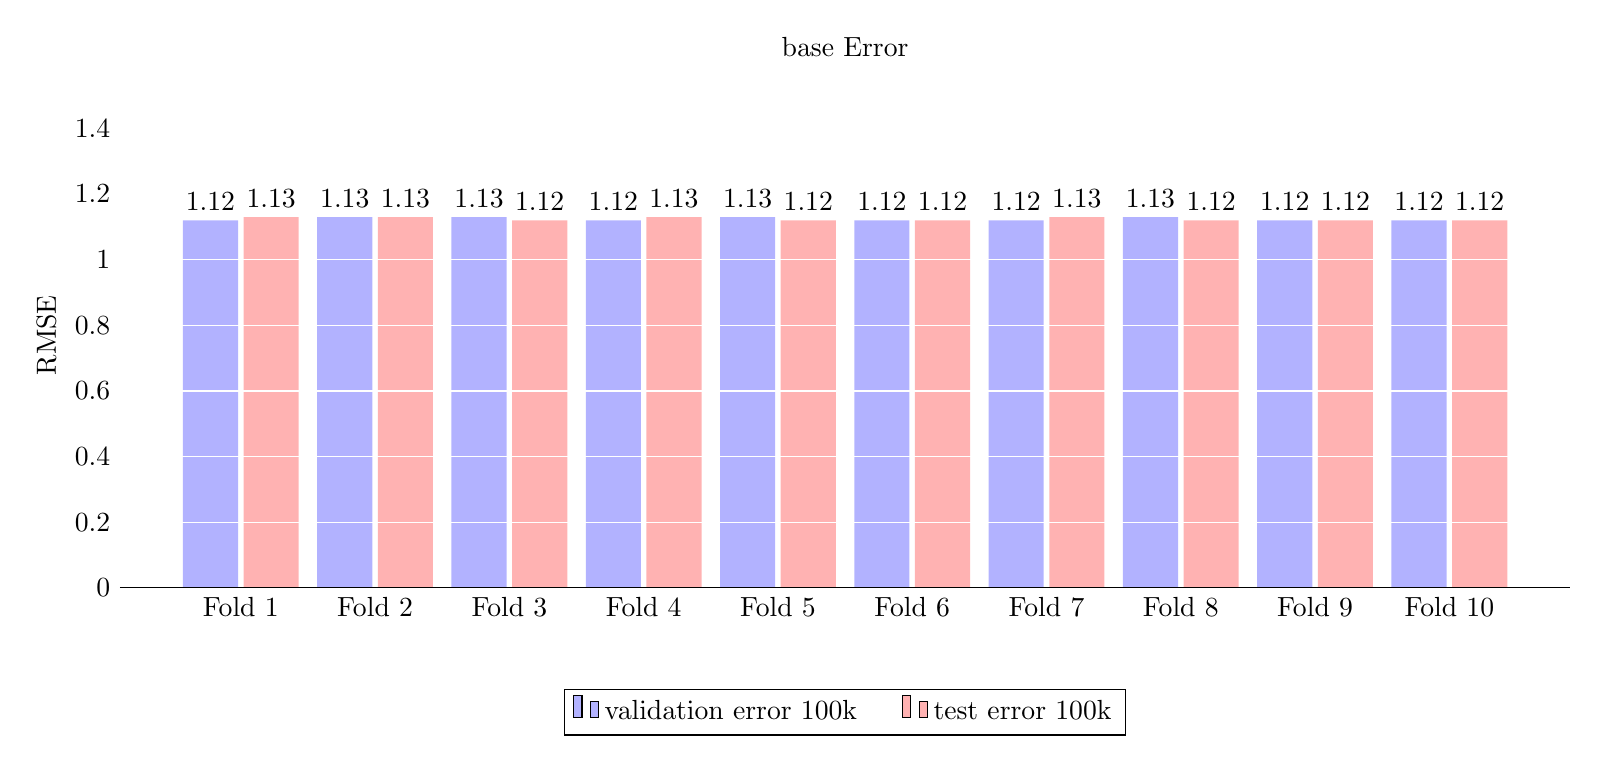
\begin{tikzpicture}
  \centering
  \begin{axis}[
        ybar, axis on top,
        title={base Error},
        height=8cm, width=20cm,
        bar width=0.7cm,
        ymajorgrids, tick align=inside,
        major grid style={draw=white},
        enlarge y limits={value=.1,upper},
        ymin=0, ymax=1.4,
        axis x line*=bottom,
        y axis line style={opacity=0},
        tickwidth=0pt,
        enlarge x limits=true,
        legend style={
            at={(0.5,-0.2)},
            anchor=north,
            legend columns=-1,
            /tikz/every even column/.append style={column sep=0.5cm}
        },
        ylabel={RMSE},
        symbolic x coords={
           Fold 1,Fold 2,
           Fold 3,Fold 4,
           Fold 5,Fold 6,
           Fold 7,Fold 8,
           Fold 9,Fold 10},
       xtick=data,
       nodes near coords={
        \pgfmathprintnumber[precision=2]{\pgfplotspointmeta}
       }
    ]
    \addplot [draw=none, fill=blue!30] coordinates {
      (Fold 1, 1.12)
      (Fold 2, 1.13)
      (Fold 3, 1.13)
      (Fold 4, 1.12)
      (Fold 5, 1.13)
      (Fold 6, 1.12)
      (Fold 7, 1.12)
      (Fold 8, 1.13)
      (Fold 9, 1.12)
      (Fold 10, 1.12)};
   \addplot [draw=none,fill=red!30] coordinates {
      (Fold 1, 1.13)
      (Fold 2, 1.13)
      (Fold 3, 1.12)
      (Fold 4, 1.13)
      (Fold 5, 1.12)
      (Fold 6, 1.12)
      (Fold 7, 1.13)
      (Fold 8, 1.12)
      (Fold 9, 1.12)
      (Fold 10, 1.12)};
    \legend{validation error 100k, test error 100k}
  \end{axis}
\end{tikzpicture}
	\end{adjustbox}
	\caption{base error from 100k dataset }
	\label{fig:base_errors}
\end{figure}

In \autoref{fig:base_errors} we have the baseline RMSE, we got this by using the average rating for the dataset as the prediction for all future ratings.

\begin{figure}[H]
	\centering
	\begin{adjustbox}{width=0.5\textwidth}
		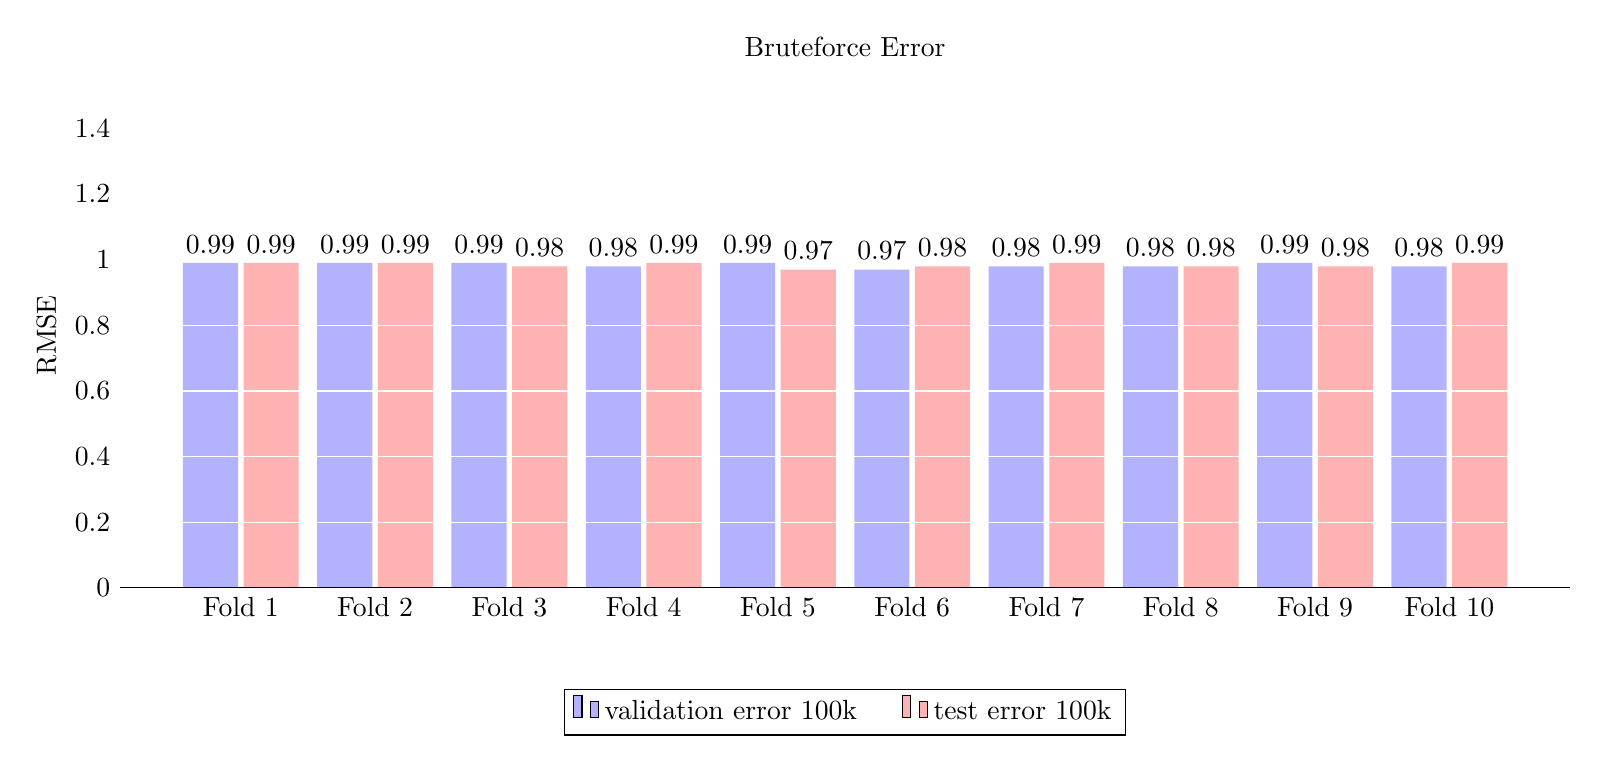
\begin{tikzpicture}
  \centering
  \begin{axis}[
        ybar, axis on top,
        title={Bruteforce Error},
        height=8cm, width=20cm,
        bar width=0.7cm,
        ymajorgrids, tick align=inside,
        major grid style={draw=white},
        enlarge y limits={value=.1,upper},
        ymin=0, ymax=1.4,
        axis x line*=bottom,
        y axis line style={opacity=0},
        tickwidth=0pt,
        enlarge x limits=true,
        legend style={
            at={(0.5,-0.2)},
            anchor=north,
            legend columns=-1,
            /tikz/every even column/.append style={column sep=0.5cm}
        },
        ylabel={RMSE},
        symbolic x coords={
           Fold 1,Fold 2,
           Fold 3,Fold 4,
           Fold 5,Fold 6,
           Fold 7,Fold 8,
           Fold 9,Fold 10},
       xtick=data,
       nodes near coords={
        \pgfmathprintnumber[precision=2]{\pgfplotspointmeta}
       }
    ]
    \addplot [draw=none, fill=blue!30] coordinates {
      (Fold 1, 0.99)
      (Fold 2, 0.99)
      (Fold 3, 0.99)
      (Fold 4, 0.98)
      (Fold 5, 0.99)
      (Fold 6, 0.97)
      (Fold 7, 0.98)
      (Fold 8, 0.98)
      (Fold 9, 0.99)
      (Fold 10, 0.98)};
   \addplot [draw=none,fill=red!30] coordinates {
      (Fold 1, 0.99)
      (Fold 2, 0.99)
      (Fold 3, 0.98)
      (Fold 4, 0.99)
      (Fold 5, 0.97)
      (Fold 6, 0.98)
      (Fold 7, 0.99)
      (Fold 8, 0.98)
      (Fold 9, 0.98)
      (Fold 10, 0.99)};
    \legend{validation error 100k, test error 100k}
  \end{axis}
  \end{tikzpicture}
	\end{adjustbox}
	\caption{bruteforce error from 100k dataset }
	\label{fig:brute_errors}
\end{figure}

\autoref{fig:brute_errors} show the RMSE for the 20 evaluations. 
This shows that with a relatively simple method, recommendations can be done better than the baseline.
\autoref{fig:brute_errors} also shows that the RMSE in most folds only have a difference of $0.01$ between validation and test sets.

\begin{figure}[H]
	\centering
	\begin{adjustbox}{width=0.5\textwidth}
		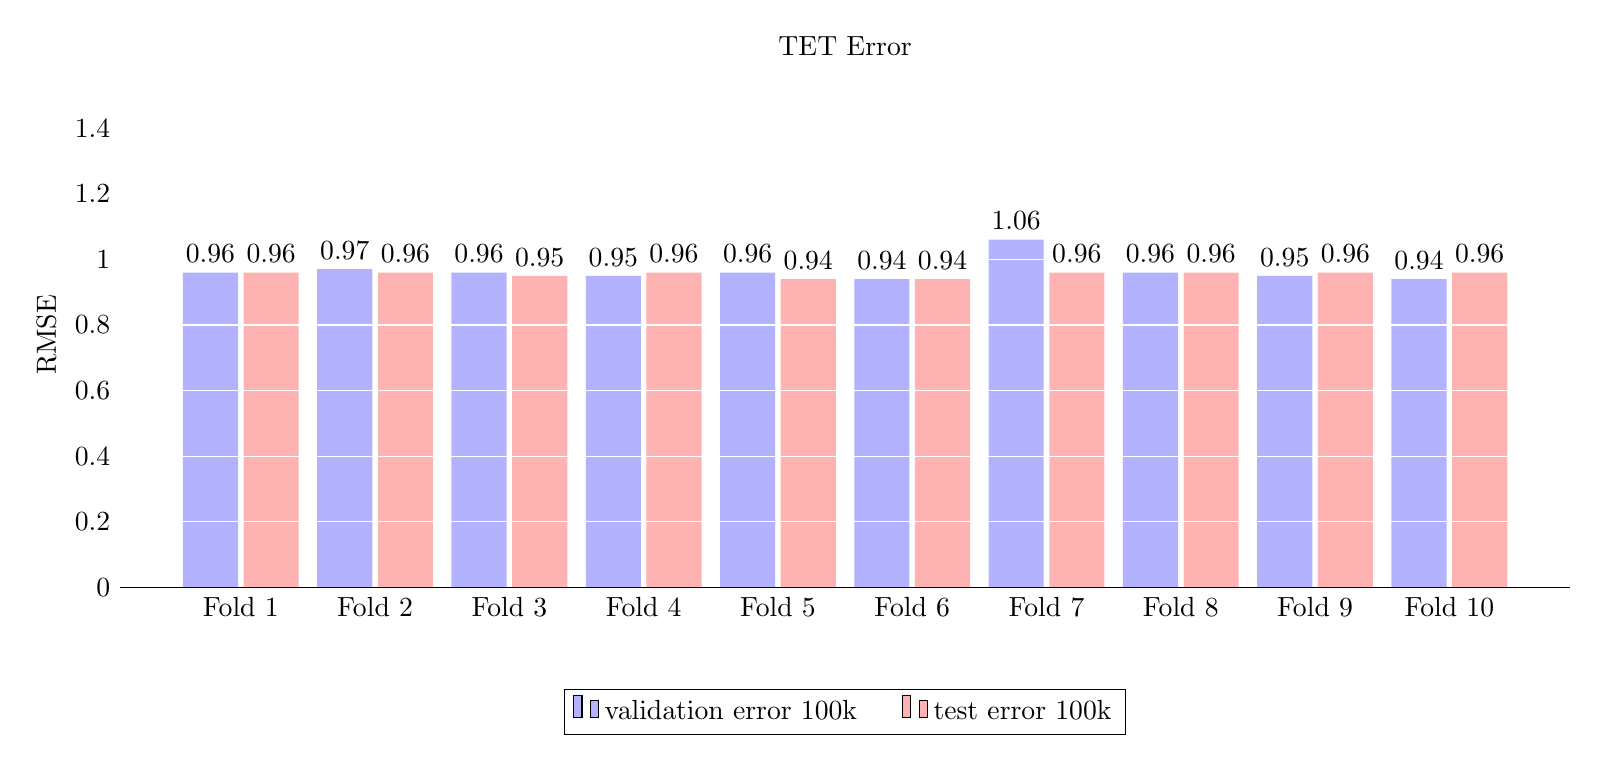
\begin{tikzpicture}
  \centering
  \begin{axis}[
        ybar, axis on top,
        title={TET Error},
        height=8cm, width=20cm,
        bar width=0.7cm,
        ymajorgrids, tick align=inside,
        major grid style={draw=white},
        enlarge y limits={value=.1,upper},
        ymin=0, ymax=1.4,
        axis x line*=bottom,
        y axis line style={opacity=0},
        tickwidth=0pt,
        enlarge x limits=true,
        legend style={
            at={(0.5,-0.2)},
            anchor=north,
            legend columns=-1,
            /tikz/every even column/.append style={column sep=0.5cm}
        },
        ylabel={RMSE},
        symbolic x coords={
           Fold 1,Fold 2,
           Fold 3,Fold 4,
           Fold 5,Fold 6,
           Fold 7,Fold 8,
           Fold 9,Fold 10},
       xtick=data,
       nodes near coords={
        \pgfmathprintnumber[precision=2]{\pgfplotspointmeta}
       }
    ]
    \addplot [draw=none, fill=blue!30] coordinates {
      (Fold 1, 0.96)
      (Fold 2, 0.97)
      (Fold 3, 0.96)
      (Fold 4, 0.95)
      (Fold 5, 0.96)
      (Fold 6, 0.94)
      (Fold 7, 1.06)
      (Fold 8, 0.96)
      (Fold 9, 0.95)
      (Fold 10, 0.94)};
   \addplot [draw=none,fill=red!30] coordinates {
      (Fold 1, 0.96)
      (Fold 2, 0.96)
      (Fold 3, 0.95)
      (Fold 4, 0.96)
      (Fold 5, 0.94)
      (Fold 6, 0.94)
      (Fold 7, 0.96)
      (Fold 8, 0.96)
      (Fold 9, 0.96)
      (Fold 10, 0.96)};
    \legend{validation error 100k, test error 100k}
  \end{axis}
  \end{tikzpicture}
	\end{adjustbox}
	\caption{Node2vec error from 100k dataset}
	\label{fig:N2V_errors}
\end{figure}

The graph in \autoref{fig:N2V_errors} shows the most promising of our results with RMSE values being as low as 0.94 . By tweaking the metadata of the training we believe that there are potential for even better recommendations.
The discrepancy between validation and test in fold 7 seems to indicate that this fold has been fitted wrongly.


\begin{figure}[H]
	\centering
	\begin{adjustbox}{width=0.5\textwidth}
		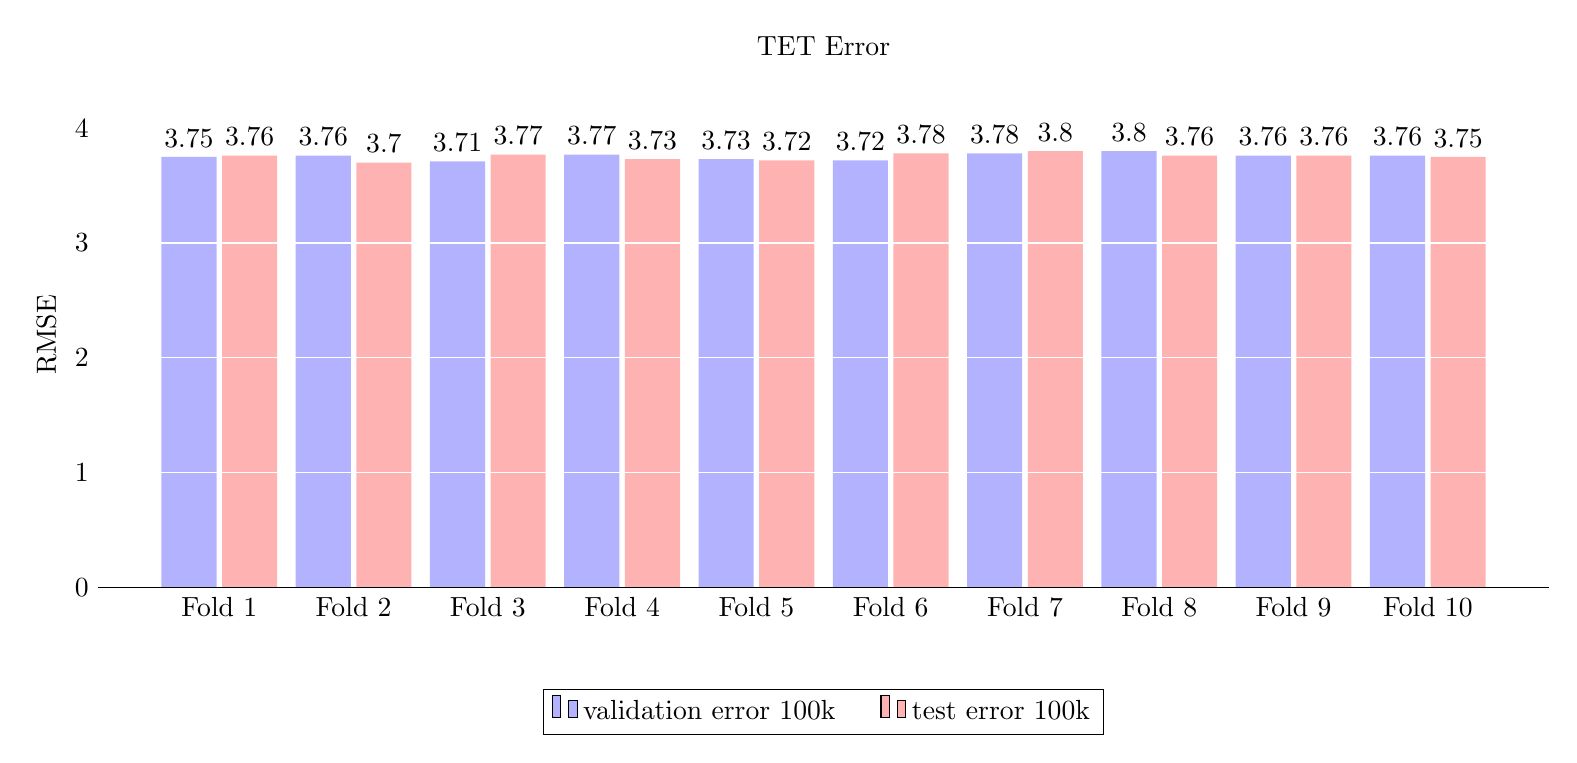
\begin{tikzpicture}
  \centering
  \begin{axis}[
        ybar, axis on top,
        title={TET Error},
        height=8cm, width=20cm,
        bar width=0.7cm,
        ymajorgrids, tick align=inside,
        major grid style={draw=white},
        enlarge y limits={value=.1,upper},
        ymin=0, ymax=4,
        axis x line*=bottom,
        y axis line style={opacity=0},
        tickwidth=0pt,
        enlarge x limits=true,
        legend style={
            at={(0.5,-0.2)},
            anchor=north,
            legend columns=-1,
            /tikz/every even column/.append style={column sep=0.5cm}
        },
        ylabel={RMSE},
        symbolic x coords={
           Fold 1,Fold 2,
           Fold 3,Fold 4,
           Fold 5,Fold 6,
           Fold 7,Fold 8,
           Fold 9,Fold 10},
       xtick=data,
       nodes near coords={
        \pgfmathprintnumber[precision=2]{\pgfplotspointmeta}
       }
    ]
    \addplot [draw=none, fill=blue!30] coordinates {
      (Fold 1, 3.75)
      (Fold 2, 3.76)
      (Fold 3, 3.71)
      (Fold 4, 3.77)
      (Fold 5, 3.73)
      (Fold 6, 3.72)
      (Fold 7, 3.78)
      (Fold 8, 3.80)
      (Fold 9, 3.76)
      (Fold 10, 3.76)};
   \addplot [draw=none,fill=red!30] coordinates {
      (Fold 1, 3.76)
      (Fold 2, 3.70)
      (Fold 3, 3.77)
      (Fold 4, 3.73)
      (Fold 5, 3.72)
      (Fold 6, 3.78)
      (Fold 7, 3.80)
      (Fold 8, 3.76)
      (Fold 9, 3.76)
      (Fold 10, 3.75)};
%   \addplot [draw=none, fill=green!30] coordinates {
%      (Sep-11,75.4064)
%      (Oct-11, 89.7961) 
%      (Nov-11,94.4597)
%      (Dec-11,76.6786) 
%      (Jan-12,77.5600) 
%      (Feb-12,78.2339)
%      (Mar-12,88.6138) 
%      (Apr-12,78.9129) };

    \legend{validation error 100k, test error 100k}
  \end{axis}
  \end{tikzpicture}
	\end{adjustbox}
	\caption{TET error from 100k dataset }
	\label{fig:tet_errors}
\end{figure}


The RMSE scores for the TETs seen in \autoref{fig:tet_errors}, are at a glance not impressive, but the RMSE scores are still better than the baseline. 
This shows potential in the framework and it might be better with more descriptive features. The advantage of recommendation with TETs, is that it can depend only on structural information.
Where the other methods we have discussed are dependent on the nearest neighbors having rated a product or movie to make a recommendation, the TETs only need movies or products that look like the movie or product you try to predict a recommendation for.

A scenario where the TETs structure should be better is with the addition of new items in the database.
We made this scenario by artificially removing any relation to all the movies in verification and test sets from all users in the traning set, and making the predictions for a single person.
The error scores will because of this be far more fluctuating.
We ran the scenario on the TETs and Node2vec.
The Node2vec's predictions should default to the users average rating because there are no other users that has rated the movies, we do not have their input to the prediction.

\begin{figure}[H]
	\centering
	\begin{adjustbox}{width=0.5\textwidth}
		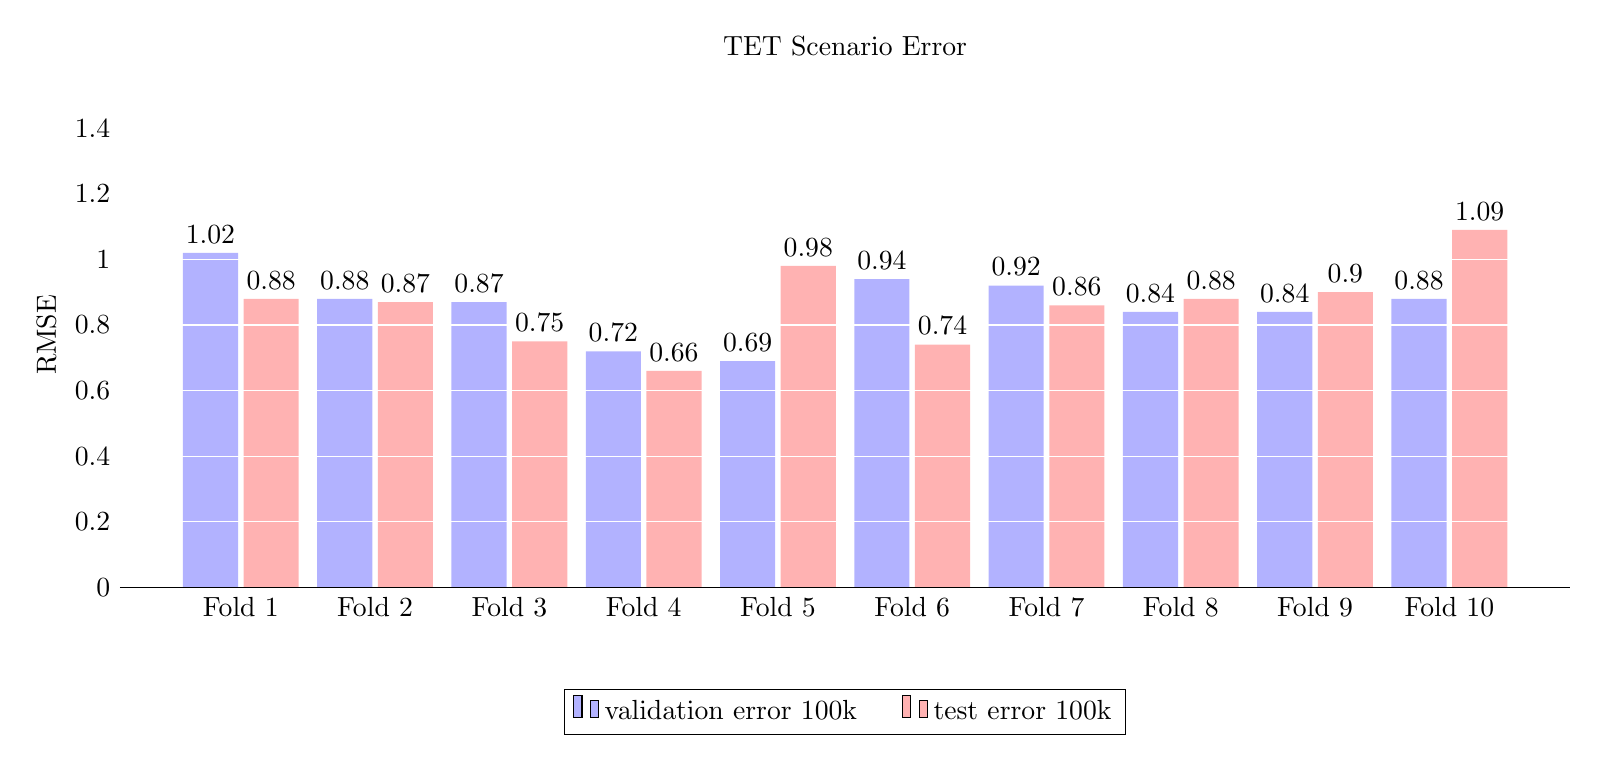
\begin{tikzpicture}
  \centering
  \begin{axis}[
        ybar, axis on top,
        title={TET Scenario Error},
        height=8cm, width=20cm,
        bar width=0.7cm,
        ymajorgrids, tick align=inside,
        major grid style={draw=white},
        enlarge y limits={value=.1,upper},
        ymin=0, ymax=1.4,
        axis x line*=bottom,
        y axis line style={opacity=0},
        tickwidth=0pt,
        enlarge x limits=true,
        legend style={
            at={(0.5,-0.2)},
            anchor=north,
            legend columns=-1,
            /tikz/every even column/.append style={column sep=0.5cm}
        },
        ylabel={RMSE},
        symbolic x coords={
           Fold 1,Fold 2,
           Fold 3,Fold 4,
           Fold 5,Fold 6,
           Fold 7,Fold 8,
           Fold 9,Fold 10},
       xtick=data,
       nodes near coords={
        \pgfmathprintnumber[precision=2]{\pgfplotspointmeta}
       }
    ]
    \addplot [draw=none, fill=blue!30] coordinates {
      (Fold 1, 1.02)
      (Fold 2, 0.88)
      (Fold 3, 0.87)
      (Fold 4, 0.72)
      (Fold 5, 0.69)
      (Fold 6, 0.94)
      (Fold 7, 0.92)
      (Fold 8, 0.84)
      (Fold 9, 0.84)
      (Fold 10, 0.88)};
   \addplot [draw=none,fill=red!30] coordinates {
      (Fold 1, 0.88)
      (Fold 2, 0.87)
      (Fold 3, 0.75)
      (Fold 4, 0.66)
      (Fold 5, 0.98)
      (Fold 6, 0.74)
      (Fold 7, 0.86)
      (Fold 8, 0.88)
      (Fold 9, 0.90)
      (Fold 10, 1.09)};
    \legend{validation error 100k, test error 100k}
  \end{axis}
  \end{tikzpicture}
	\end{adjustbox}
	\caption{TET scenario error from 100k dataset}
	\label{fig:tet_scenario_errors}
\end{figure}

\begin{figure}[H]
	\centering
	\begin{adjustbox}{width=0.5\textwidth}
		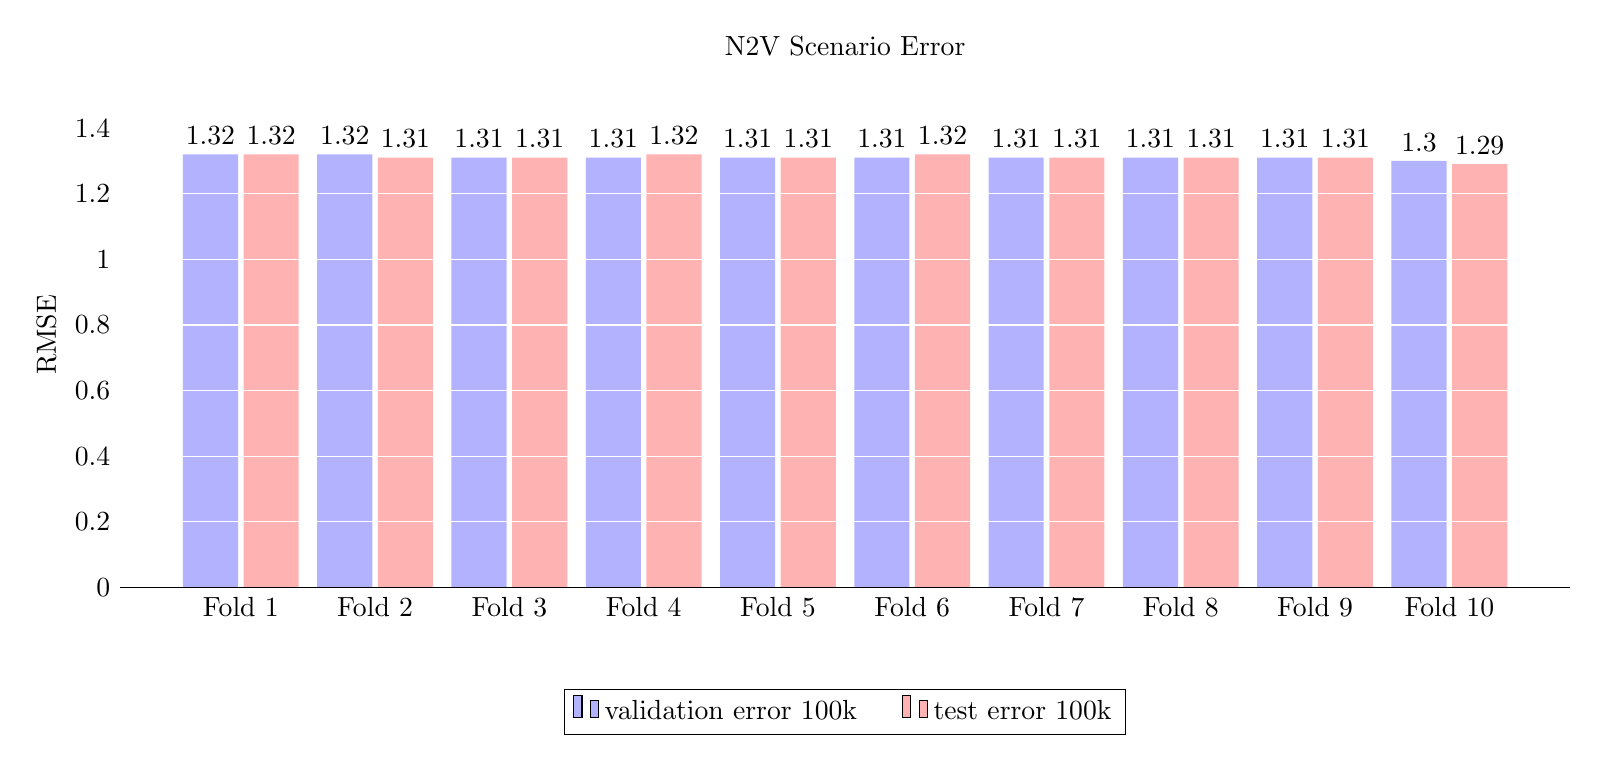
\begin{tikzpicture}
  \centering
  \begin{axis}[
        ybar, axis on top,
        title={N2V Scenario Error},
        height=8cm, width=20cm,
        bar width=0.7cm,
        ymajorgrids, tick align=inside,
        major grid style={draw=white},
        enlarge y limits={value=.1,upper},
        ymin=0, ymax=1.4,
        axis x line*=bottom,
        y axis line style={opacity=0},
        tickwidth=0pt,
        enlarge x limits=true,
        legend style={
            at={(0.5,-0.2)},
            anchor=north,
            legend columns=-1,
            /tikz/every even column/.append style={column sep=0.5cm}
        },
        ylabel={RMSE},
        symbolic x coords={
           Fold 1,Fold 2,
           Fold 3,Fold 4,
           Fold 5,Fold 6,
           Fold 7,Fold 8,
           Fold 9,Fold 10},
       xtick=data,
       nodes near coords={
        \pgfmathprintnumber[precision=2]{\pgfplotspointmeta}
       }
    ]
    \addplot [draw=none, fill=blue!30] coordinates {
      (Fold 1, 1.32)
      (Fold 2, 1.32)
      (Fold 3, 1.31)
      (Fold 4, 1.31)
      (Fold 5, 1.31)
      (Fold 6, 1.31)
      (Fold 7, 1.31)
      (Fold 8, 1.31)
      (Fold 9, 1.31)
      (Fold 10, 1.30)};
   \addplot [draw=none,fill=red!30] coordinates {
      (Fold 1, 1.32)
      (Fold 2, 1.31)
      (Fold 3, 1.31)
      (Fold 4, 1.32)
      (Fold 5, 1.31)
      (Fold 6, 1.32)
      (Fold 7, 1.31)
      (Fold 8, 1.31)
      (Fold 9, 1.31)
      (Fold 10, 1.29)};
    \legend{validation error 100k, test error 100k}
  \end{axis}
  \end{tikzpicture}
	\end{adjustbox}
	\caption{Node2vec scenario error from 100k dataset}
	\label{fig:N2V_scenario_errors}
\end{figure}

From this scenario we can clearly see that the TET comparison and predictions (\autoref{fig:tet_scenario_errors}), are better than the predictions made by Node2Vec (\autoref{fig:N2V_scenario_errors}).
Fold 4 for the in \autoref{fig:N2V_scenario_errors} is the best trained for the scenario.
This fold shows a difference between validation and test of 0.03 but at the lowest it has a RMSE at 1.08.
The RMSE for the TET predictions  as shown in \autopageref{fig:tet_scenario_errors} only has two folds were either validation or test has a RMSE of more than 1.
All other folds has a RMSE below one, but the predictions has some uncertainty between validation and test.
